\textbf{Data4Help Mobile App:}

The Mobile app should offer an easy interface aiming a user friendly experience of the customers. If should be possible to open a menu to navigate through the sub-sections. All the main functions (i.e. see history of activities, see account information) should be easy to access from any sub-section of the app. 
Descriptions of the pages has to be brief and concise.
To see the details of the statistics there should be an info button that shows detailed description about the related data.
If subscribed to the AutomatedSOS service, there should be a page showing the active controls on the user.
In case of using the Track4Run service, there is also the possibility to see the map of a programmed run and seeing on the map all the participants, and their positions. More detailed info of the runners can be shown by tapping on their icon on the map.

The application must follow a proper design for every different mobile operating system:
\begin{itemize}
    \item Android - \vspace{0.3cm} Material Design
    \item iOS - \vspace{0.3cm} Human Interfaces
\end{itemize}
The application should support all the screen resolutions available and optimize the item placement on the screen in the same way for every compatible device.
\newline
The user can configure the graphic of the widget visible from the Smartwatch only using the Mobile App component.

\begin{figure}
\centering
\begin{minipage}{.5\textwidth}
  \centering
  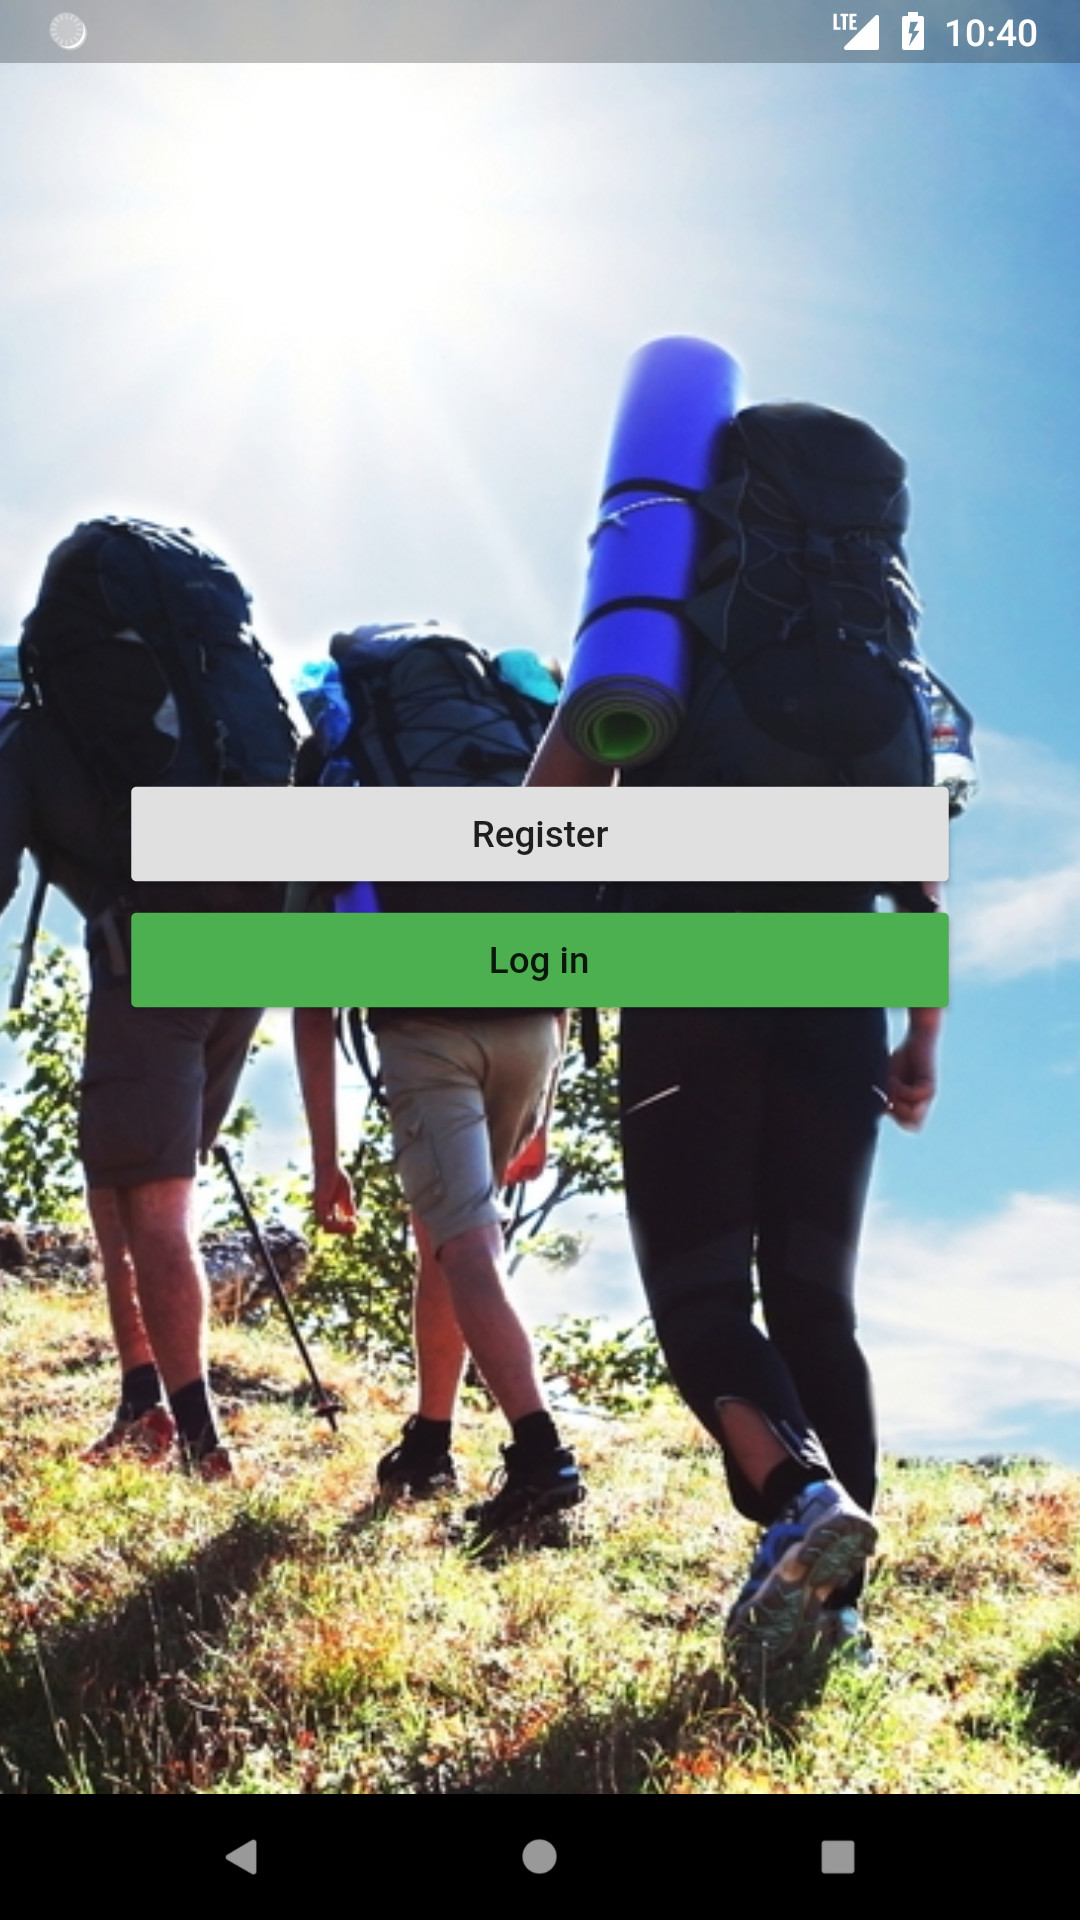
\includegraphics[width=.5\linewidth]{assets/mockup/flutter_01.jpg}
  \caption{Login and Registration}
\end{minipage}%
\begin{minipage}{.5\textwidth}
  \centering
  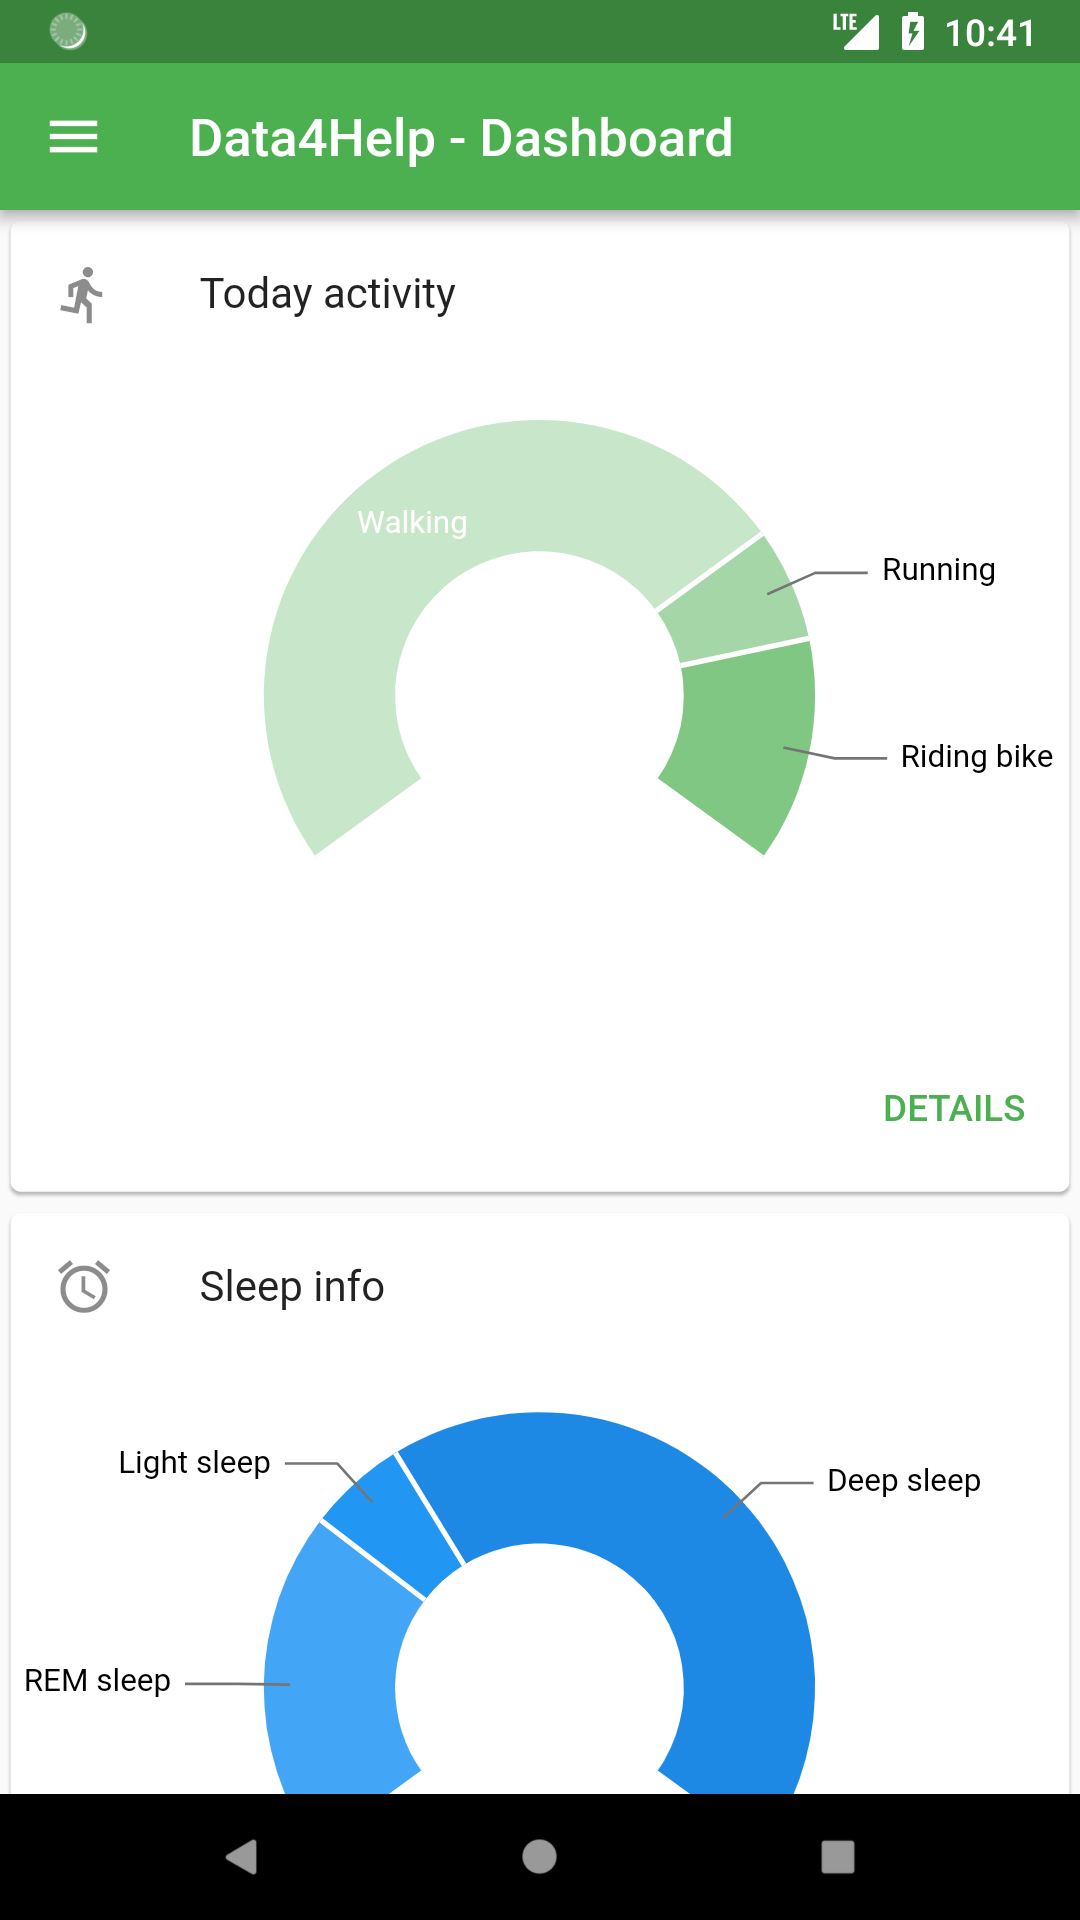
\includegraphics[width=.5\linewidth]{assets/mockup/flutter_02.png}
  \caption{Dashboard}
\end{minipage}
\end{figure}
\begin{figure}
\centering
\begin{minipage}{.5\textwidth}
  \centering
  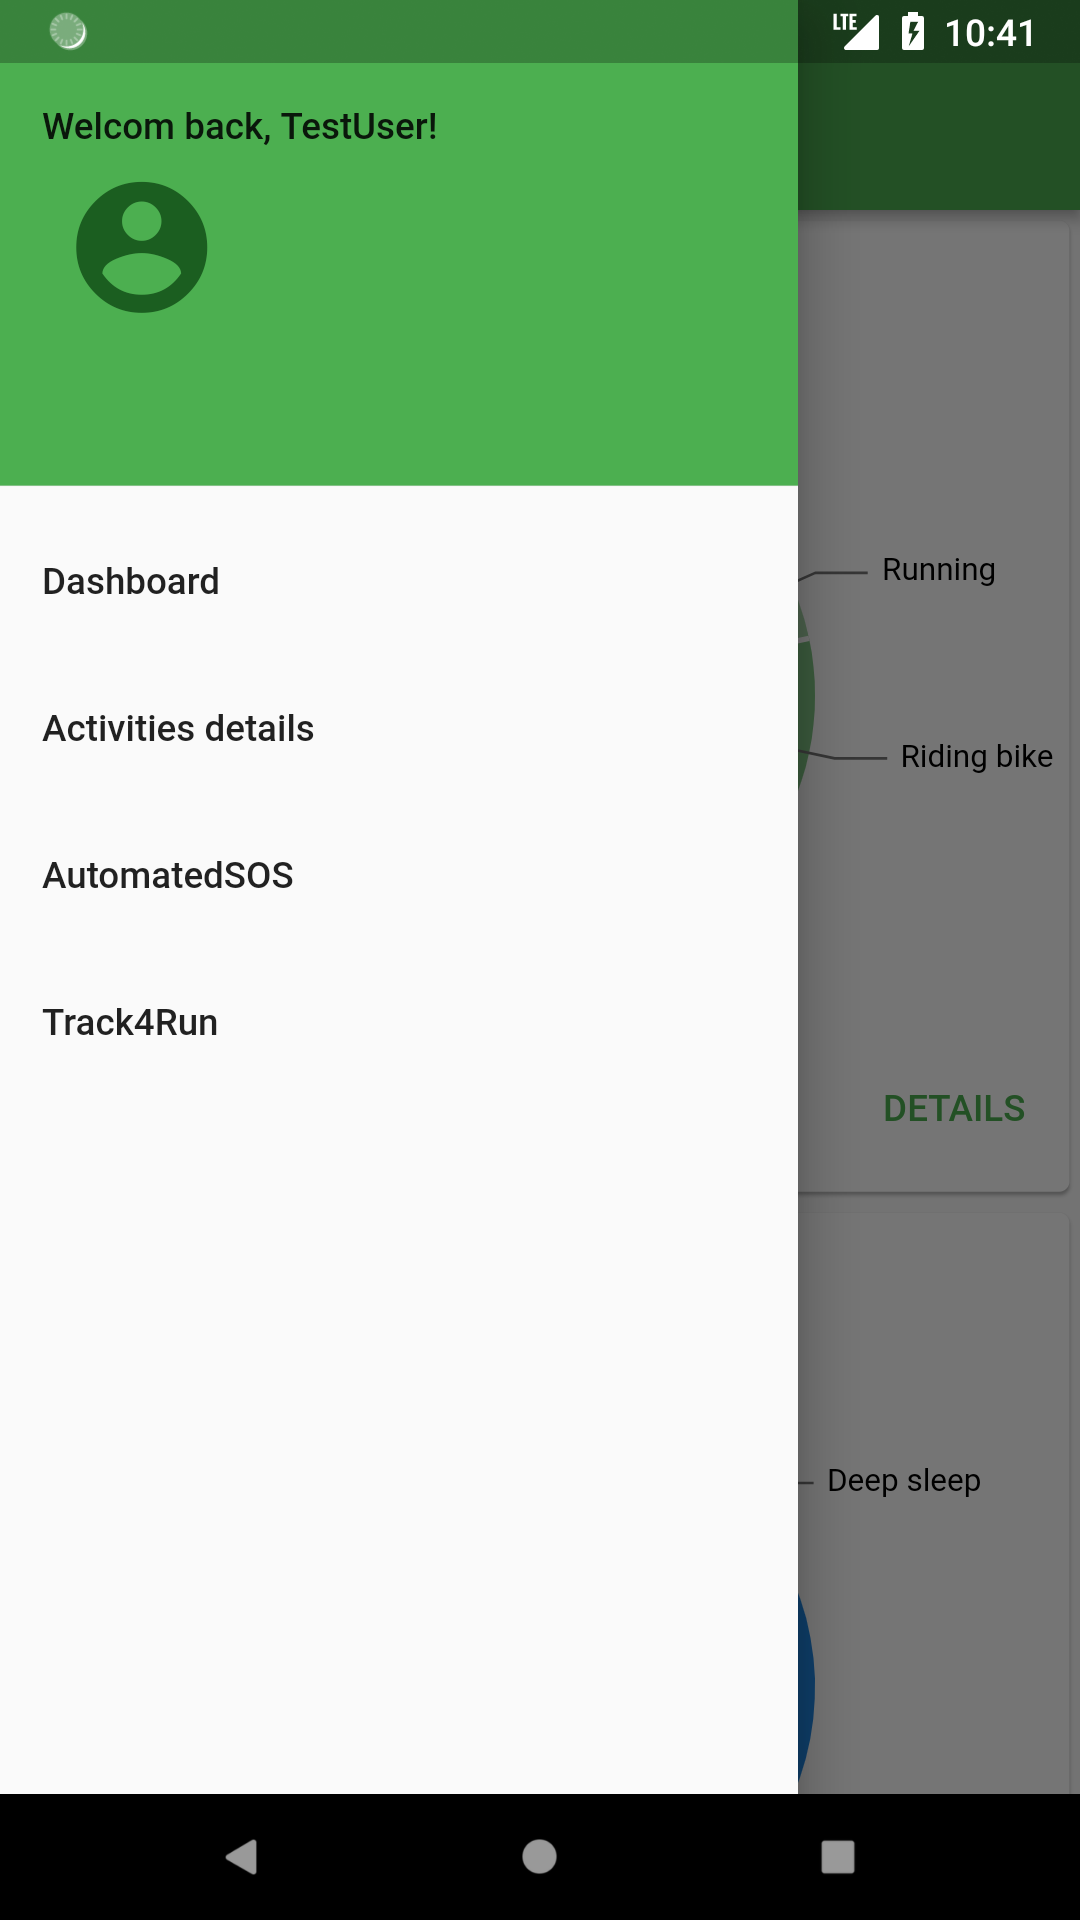
\includegraphics[width=.5\linewidth]{assets/mockup/flutter_03.png}
  \caption{Menu}

\end{minipage}%
\begin{minipage}{.5\textwidth}
  \centering
  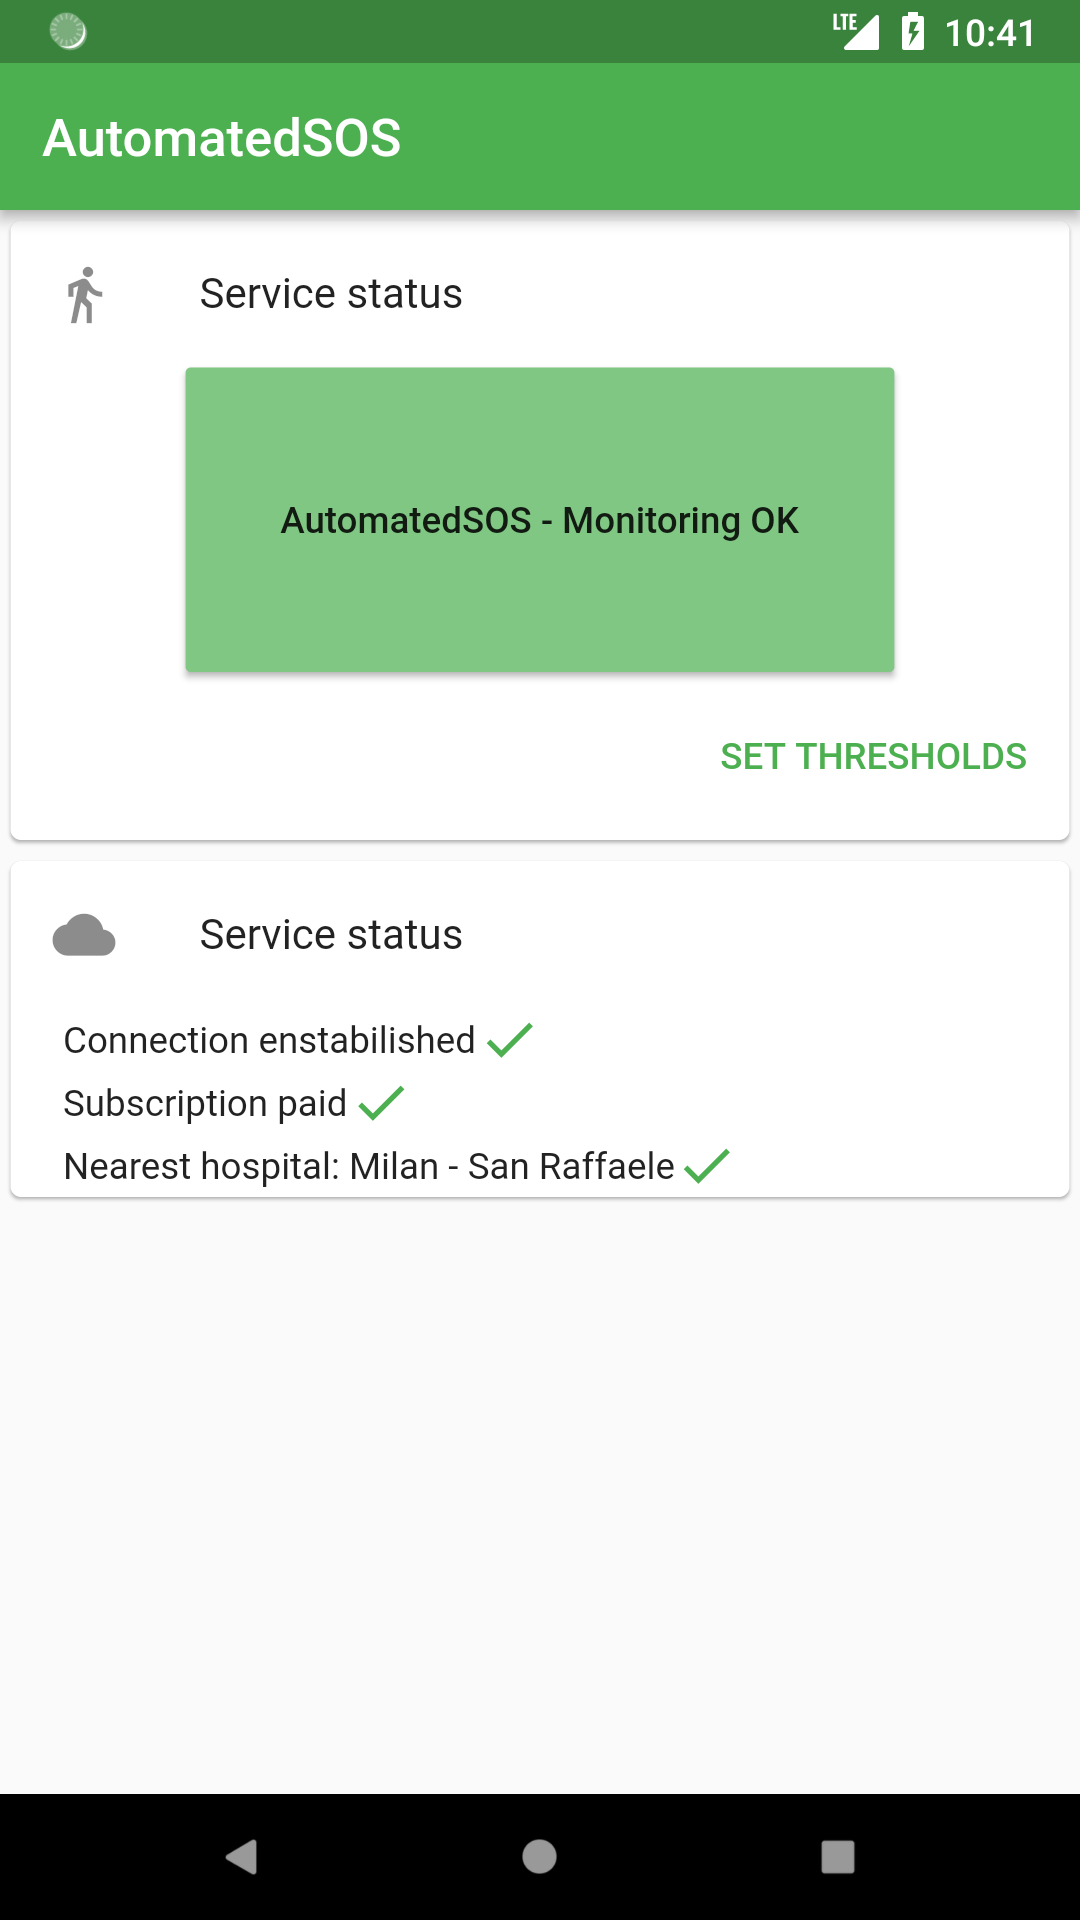
\includegraphics[width=.5\linewidth]{assets/mockup/flutter_04.png}
  \caption{AutomatedSOS}

\end{minipage}
\end{figure}
\begin{figure}
\centering
\begin{minipage}{.5\textwidth}
  \centering
  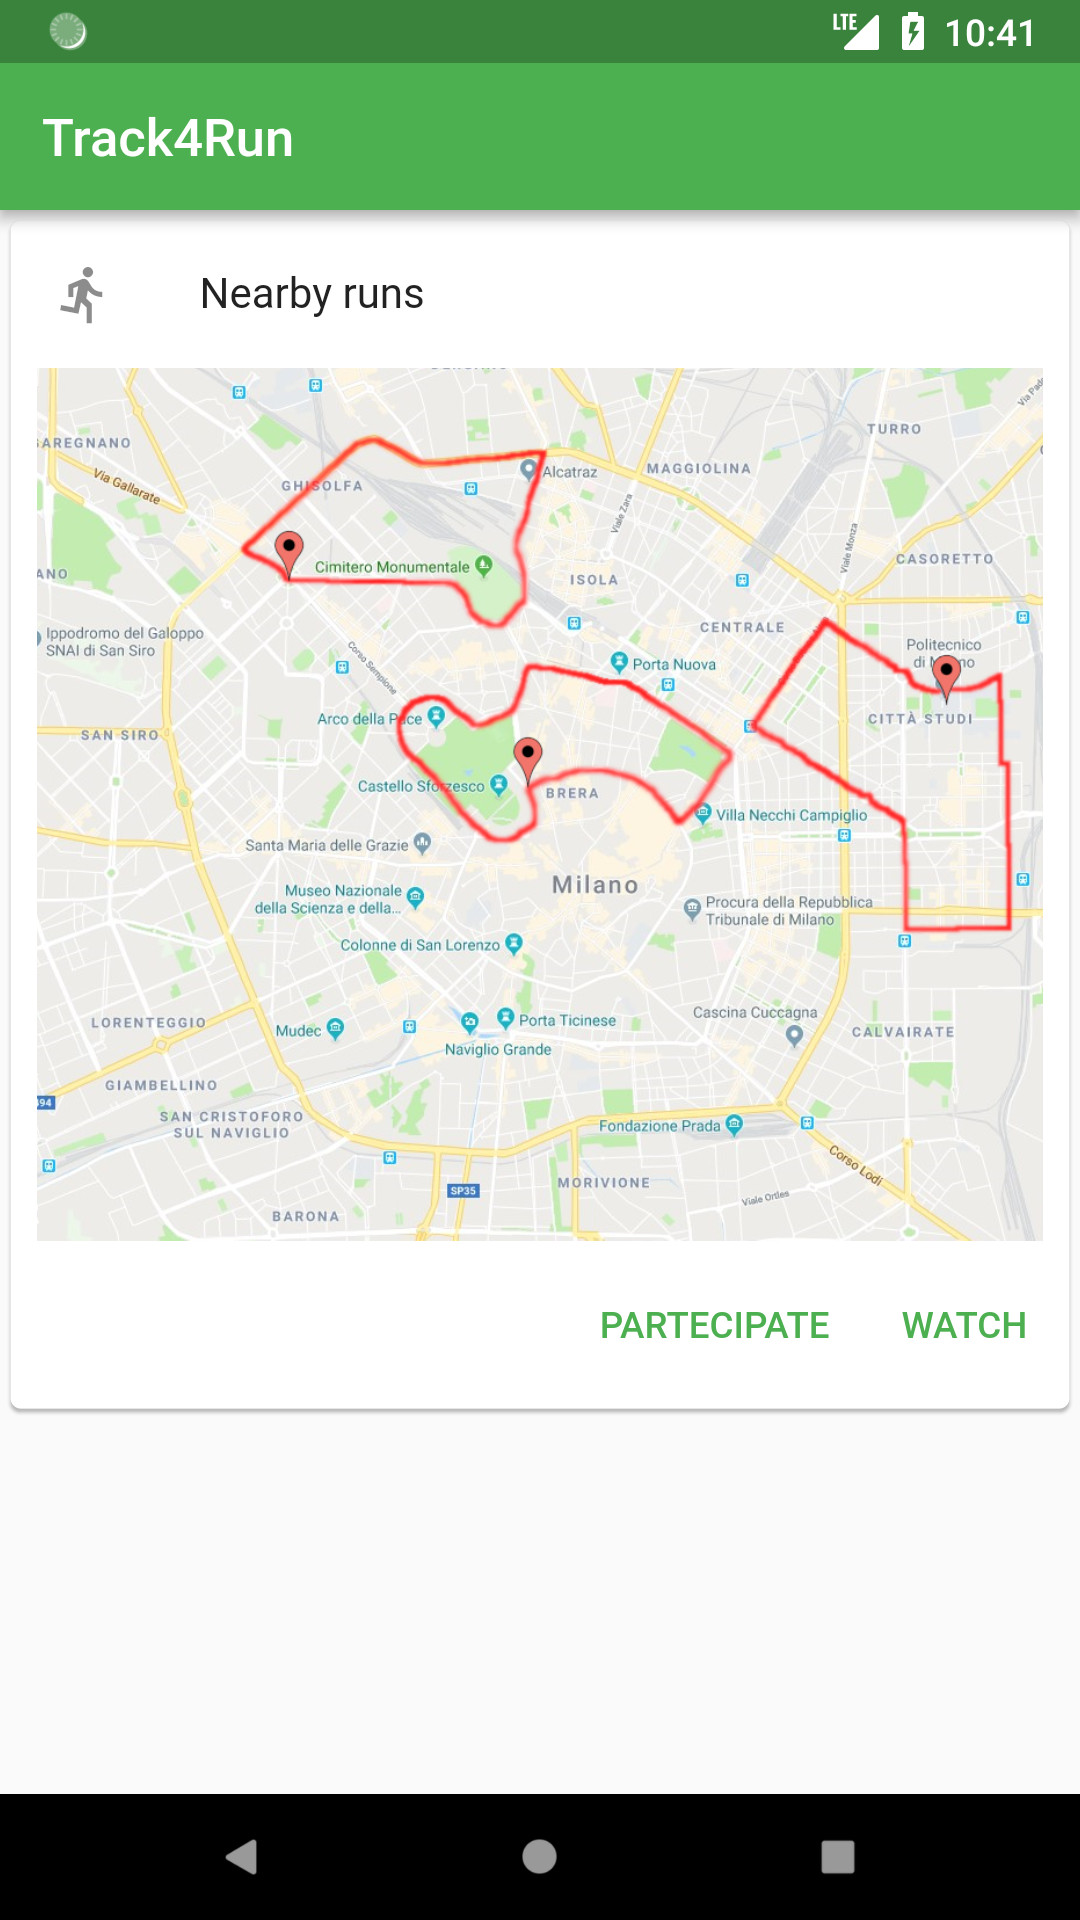
\includegraphics[width=.5\linewidth]{assets/mockup/flutter_05.jpg}
  \caption{Track4Run}

\end{minipage}%
\begin{minipage}{.5\textwidth}
  \centering
  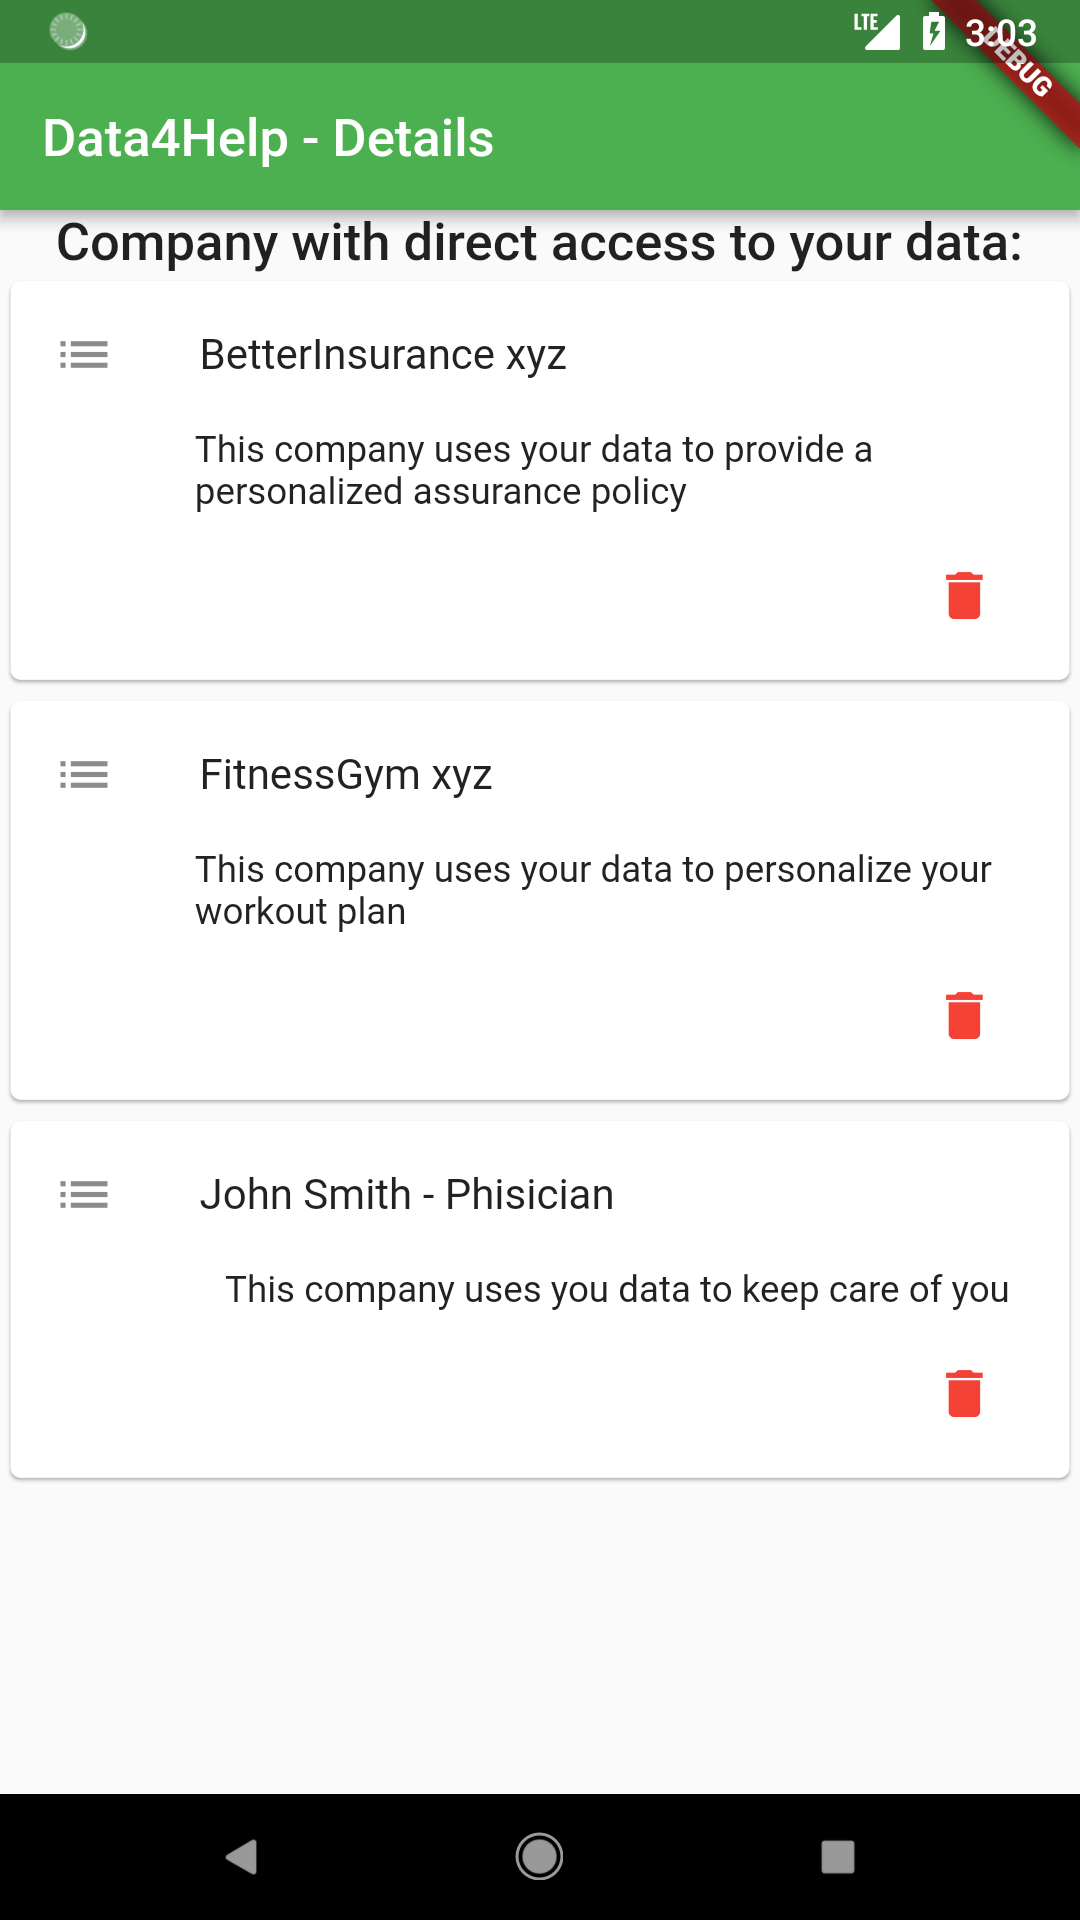
\includegraphics[width=.5\linewidth]{assets/mockup/flutter_06.png}
  \caption{Company requests for monitoring}

\end{minipage}
\end{figure}

\textbf{Data4Help SmartWatch App} :
The Smartwatch app should provide \textbf{widgets} that let the customer see their daily activity.
There should be one widget for every type of data acquired by the device:
\begin{itemize}
    \item Sleep monitoring 
    \item Heart rate
    \item Blood pressure
\end{itemize}
The user can receive notifications about his activities in the Smartwatch and delete them through it.
\newline

\textbf{Data4Help WebSite}: The Website should offer an easy interface aiming a user friendly experience for the subscribed companies. The main menu should be visible on the top of the page, and must be used to navigate through the sub-sections. All the main functions (i.e. acquired data, account information, etc) should be accessible from any sub-section of the web page. 
Descriptions of the pages have to be clear and exhaustive.
\newline

\textbf{Data4Help Core:} This component does not have a user interface since it is intended to be accessible only by the qualified staff that manages it. 